\chapter{Simultaneous Localisation and Mapping}

Simultaneous Localisation and Mapping, kurz SLAM, ist das Problem der Auswertung einer unbekannten Umgebung und Erstellung einer Map, während gleichzeitig die lokale Position innerhalb dieser Map bestimmt wird. Die Lösung dieses SLAM Problems war vorallem in der Robotik eine fundamentale Aufgabe der letzten zwei Jahrzehnte. Dabei ist SLAM ein Alltagsproblem: Das Problem der räumlichen Erkundung. Jeder Mensch und jedes Tier hat dieses Verfahren gemeistert und benutzt es unterbewusst zur Navigation in unserer Realität. Die Lösung dieses Problems, wenn es für einen Roboter automatisiert ausgeführt werden soll, ist dagegen sehr komplex. Durch das Meistern dieser Technik kann man Roboter wirklich autonom steuern. 
Bei SLAM wird die Bewegung des Objekts an sich durch den Raum und die Position aller zur positionsbestimmung notwendigen Merkmale berechnet, ohne auf vorheriges Wissen, über Position oder Lage im Raum, Kenntniss zu haben. (vgl. \cite{slam} S. 1-2) 

Dabei benötigt der Roboter mindestens einen exterozeptiven Sensor um äußere Informationen zu sammeln.
SLAM besteht aus drei grundlegenden Operationen, die iterativ pro Zeitintervall ausgeführt werden.

\textbf{Der Roboter bewegt} sich und erreicht eine neue Position in der Umwelt. Diese Bewegung erzeugt, durch unvermeidbares Rauschen und Fehler, Ungewissheit über die wirkliche Position des Roboters. Eine automatisierte Lösung benötigt ein mathematisches Modell für diese Bewegung. Dies ist das \glqq\textit{Motion Model}\grqq

\textbf{Der Roboter entdeckt neue Features} in seiner Umgebung, welche in die Umgebungskarte aufgenommen werden müssen. Diese Features heißen \glqq Landmarks\grqq . Da die Position der Landmarks, durch Fehler in den exterozeptiven Sensoren und die Position des Roboters ungewiss ist, müssen diese beiden Faktoren passend arrangiert werden. Eine automatisierte Lösung benötigt ein mathematisches Modell, das die Position der Landmarks anhand er Sensordaten bestimmt. Dies ist das \glqq \textit{Inverse Oberservation Model} \grqq .

\textbf{Der Roboter entdeckt Landmarks, die schon gemappt wurden} und verwendet diese um seine eigene Position, sowie die aller Landmarks zu korrigieren. Diese Operation reduziert die Unsicherheit über den Standort des Roboters, sowie der Landmarks. Die automatisierte Lösung erfordert ein mathemathisches Modell, um die Werte der Messungen aus den prognostizierten Positionen der Landmarks und der Position des Roboters zu berechnen. Dies ist das \glqq \textit{Direct Observation Model} \grqq

Mit diesen drei Modellen ist es möglich eine automatisierte Lösung für SLAM zu entwerfen. Diese Lösung muss diese drei Modelle verbinden und alle Daten korrekt und oganisiert halten, sowie die korrekten Entscheidungen bei jedem Schritt machen. (vgl. \cite{ekf_slam} S.2-3)

Eine erfolgreiche Lösung des SLAM Problems setzt weiterhin die Lösung des \glqq Loop Closure Detection\grqq Problems vorraus. Dabei müssen bereits besuchte Orte in der beliebig großen Map erkannt werden. Wegen der möglichen Komplexität von großen Maps ist es auch eins der größten Hindernisse, wenn es um die Skalierbarkeit der Lösung geht. Wichtig ist, dass die Loop Closure Detection keine Falsch-Positiven Ergebnisse liefert, da dies die Integrität und Korrektheit der kompletten Map beeinflusst. (vgl. \cite{ar_slam} S.4)


\begin{figure}[H]
	\centering
	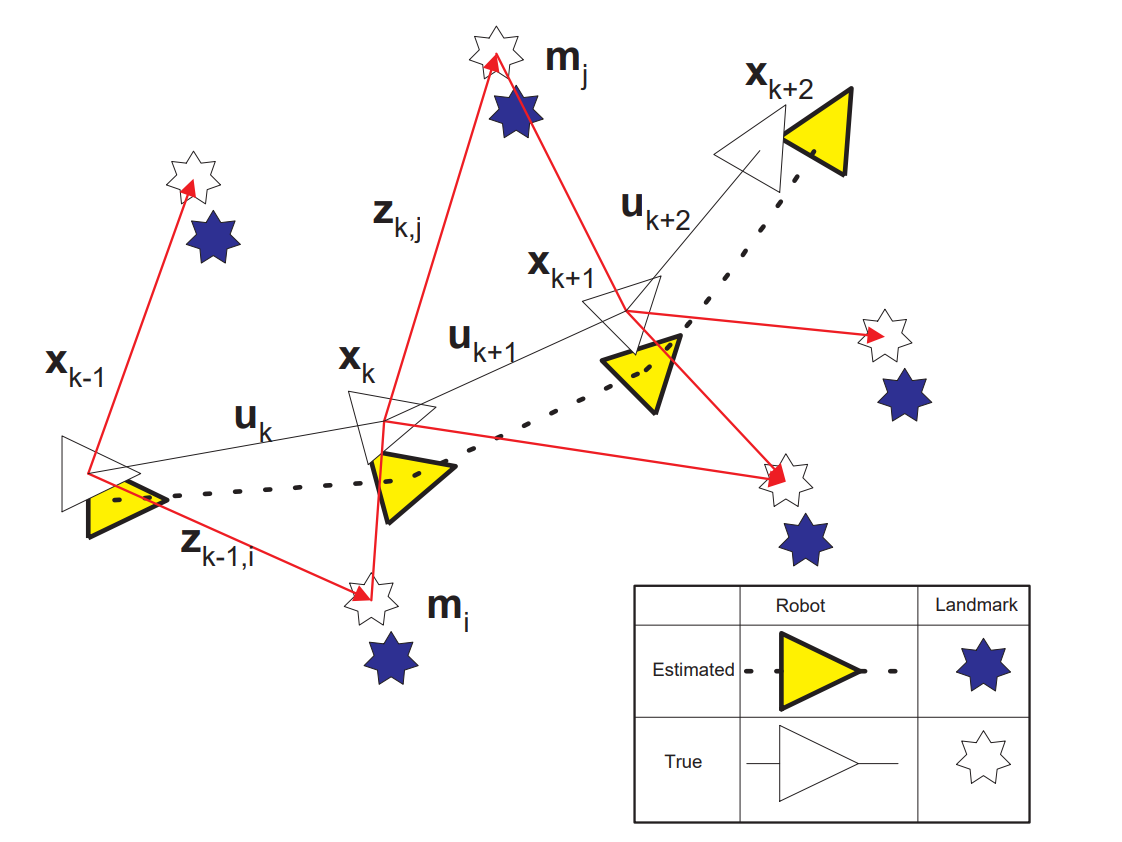
\includegraphics[scale=0.35]{slam_problem.png}
	\caption{Das SLAM Problem: Die wahren absoluten Positionen der extrahierten Features sind nie wirklich bekannt. Bildquelle \cite{slam}}
\end{figure} 

Wie in Abbildung 3.1. erkennbar ist, bewegt sich ein Roboter durch eine unbekannte Umgebung und nimmt mit seinem Sensor Features der näheren Objekte (Landmarks) auf. Wobei \large\textbf{x}\normalsize\textit{k} der Vektor des Roboters,  \large\textbf{u}\normalsize\textit{k} der Bewegungsvektor, \large\textbf{m}\normalsize\textit{i} der Vektor des Landmarks und \large\textbf{z}\normalsize\textit{ik} die Oberservation eines Landmarks durch den Roboter zur Zeit \large\textit{k }\normalsize sind. Wie man sehen kann, ist der Fehler zwischen echten und geschätzten Landmarks, bei allen geschätzten Landmarks ähnlich, was an der initialen Betrachtung der Umgebung liegt. Zu diesem Zeitpunk wird nur das erste Feature erkannt. Daraus kann man schließen, dass die Fehler in der Schätzung der Landmarkpositionen korrelieren. Praktisch bedeutet dies, dass die relative Position zweier Landmarks, \large\textbf{m}\normalsize\textit{i} - \large\textbf{m}\normalsize\textit{j} zueinander sehr genau sein kann, auch wenn die absolute Position sehr ungenau ist. 

Je mehr Landmarks in das Modell aufgenommen werden, desto gleichbleibend besser wird das Modell der relativen Positionen, egal wie sich der Roboter bewegt. Dieser Prozess wird in Abbildung 3.2. veranschaulicht.

\begin{figure}[H]
	\centering
	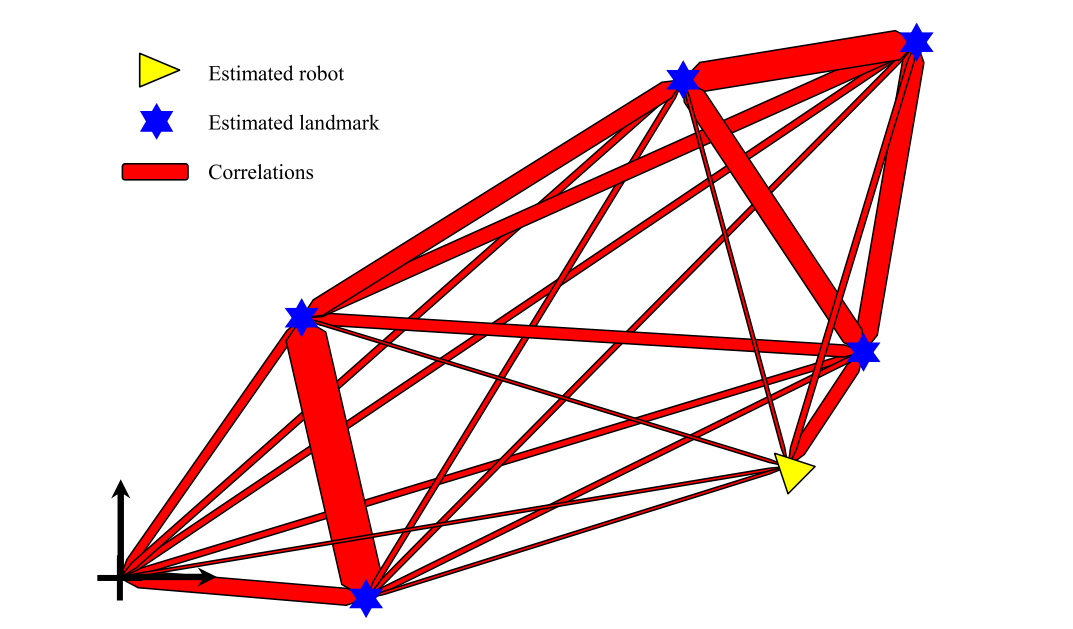
\includegraphics[scale=0.5]{slam_springs.png}
	\caption{Die Landmarks sind durch Federn verbunden, welche die Korrelation zwischen ihnen darstellen.  Bildquelle \cite{slam}}
\end{figure}  

Während sich der Roboter durch die Umgebung bewegt, werden die Korrelationen stetig aktualisiert. Je mehr Beobachtungen über die Umwelt gemacht werden, desto steifer werden die Federn in diesem Modell. Im Nachhinein werden neue Beobachtungen von Landmarks durch das ganze Netzwerk propagiert und je nach Input, kleinere oder größere Anpassungen vorgenommen.

Lösungen für das SLAM Problem benötigen eine angemessene Repräsentation für die Observierungen der Landmarks, welche eine konsistente und schnelle Berechnung ermöglichen. Die geläufigste Repräsentation besteht in der Form einer Zustandsraumdarstellung mit Gaußschen Rauschen, was zur Verwendung des \glqq Extended Kalman Filter\grqq (EKF) führt. (vgl. \cite{slam} S. 2-4)

Weitere gängige Lösungen für das SLAM Problem sind \glqq Maximum Likelihood Techniques \grqq, \glqq Sparse Extended Information Filters \grqq (SEIFs) und \glqq Rao Blackwellized Particle Filters\grqq  (RBPFs). 
 (vgl. \cite{rao} S. 2)

\section{Extended Kalman Filter - SLAM}
Der Kalman Filter ist eine Schätzfunktion für das \glqq linear-quadratic-problem\grqq , welches das Problem der Schätzung des augenblicklichen Zustands eines linearen dynamischen Systems, gestört durch weißes Rauschen, darstellt. Der Kalman Filter wird auch dazu benutzt um die mögliche Zukunft von dynamischen Systemen vorherzusagen, die von Menschen nicht kontrolliert werden können, wie zum Beispiel die Flugbahn von Himmelskörpern, oder der Kurs von gehandelten Rohstoffen. (vgl. \cite{ekf} S.1)

Der Kalman Filter besteht aus drei Schritten. Zuerst wird eine Messung vorhergesagt, welche dann mit der realen Messung verglichen wird. Die resultierende Differenz wird mit der Varianz der Messung gewichtet, um daraus eine neue Schätzung des Zustands zu erhalten. (vgl. \cite{slam_studi} S.13) Der Kalman Filter lässt sich jedoch nur auf lineare Systeme anwenden. Der EKF verwedet für die Vorhersage der Messungen und der Zustände hingegen nichtlineare Funktionen. (vgl. \cite{slam_studi} S.16-17)

Bei Extended Kalman Filter - SLAM ist die Map ein großer Stapel an Vektor und Sensordaten, sowie Zuständen von Landmarks.

\begin{equation}
  x =  \begin{bmatrix}
		R\\
		M
     	\end{bmatrix}
     = \begin{bmatrix}
		R\\
		L_1\\
		...\\
		L_n
     	\end{bmatrix}
\end{equation}

\( R\) ist der Zustand des Roboters und \( M = (L_1, ..., L_n)\)  ist das Set an Zuständen der Landmarks.
Bei EKF wird die Map durch eine gaußsche Variable modelliert, die den Mittelwert und die Kovarianzmatrix des Zustandsvektors verwendet, die jeweils durch \(\overline{x}\) und \(P\) beschrieben werden. Das Ziel ist es die Map \{\(\overline{x}, P\)\} zu allen Zeiten auf dem aktuellsten Stand zu halten.


\begin{equation}
  \overline{x} =  
  		\begin{bmatrix}
		\overline{R}\\
		\overline{M}
     	\end{bmatrix}
     = 
     	\begin{bmatrix}
		\overline{R}\\
		\overline{L_1}\\
		...\\
		\overline{L_n}
     	\end{bmatrix}
     	\quad\quad
     P = 
     	\begin{bmatrix}
		P_{RR} & P_{RM}\\
		P_{MR} & P_{MM}
     	\end{bmatrix}
     = 
     	\begin{bmatrix}
		P_{RR} & P_{RL1} & ... & P_{RLn}\\
		P_{L1R} & P_{L1L1} & ... & P_{L1Ln}\\
		... & ... & ... & ... \\
		P_{LnR} & P_{LnL1} & ... & P_{LnLn}
     	\end{bmatrix}
\end{equation}

Diese Map, die als stochastische Map bezeichnet wird, wird durch die Vorhersage- und Korrekturprozesse des EKF in Stand gehalten. Um eine echte Erkundung der Umgebung zu erreichen, wird der EKF Algorithmus mit einem extra Schritt der Landmark Erkennung und Initialisierung gestartet, bei dem neue Landmarks der Map hinzugefügt werden. Die Landmark Initialisierung erfolgt durch eine Umkehrung der Bewertungsfunktion und der Verwendung dieser und der Ableitungsmatrix, um die beobachteten Landmarks und die benötigten Co- und Crossvarianzen für den Rest der Map zu berechnen. Diese Beziehungen werden dann an den Zustandsvektor und die Kovarianzmatrix angehängt. (vgl. \cite{ekf_slam} S.6-7)

Eine zentrale Einschränkung des EKF basierten SLAM Ansatzes ist die Komplexität der Berechnung. Sensor-Updates benötigen Zeit, quadratisch zur Anzahl der Landmarks \(K\), die zu berechnen sind. Diese Komplexität ergibt sich aus der Tatsache, dass die vom Kalman-Filter verwaltete Kovarianzmatrix \(O(K²)\) Elemente enthält, die alle aktualisiert werden müssen, auch wenn nur ein einzelnes Landmark beobachtet wurde. Diese Komplexität limitiert die Anzahl an Landmarks, die durch diesen Ansatz verarbeitet werden konnen, auf ein paar Hunderte, während natürliche Umgebungsmodelle häufig Millionen von Features enthalten. (vgl. \cite{ekf_problems} S.1)

\url{http://www.iri.upc.edu/people/jsola/JoanSola/objectes/curs_SLAM/SLAM2D/SLAM%20course.pdf}

\section{ORB-SLAM}
TODO

\url{http://www.willowgarage.com/sites/default/files/orb_final.pdf}

https://arxiv.org/pdf/1502.00956.pdf
https://arxiv.org/pdf/1610.06475.pdf

\section{FAST-SLAM}

Fast-SLAM (Fast SLAM 1.0) zerlegt das SLAM-Problem in ein Lokalisierungsproblem des Roboters und eine Reihe von Landmark Schatzungsproblemen, die auf der Schätzung der Roboterposition beruhen. Fast-SLAM verwendet einen modifizierten Partikelfilter zur Schätzung der \glqq A-posteriori-Wahrscheinlichkeit\grqq  für die Roboterposition. Partikelfilter sind vom Prinzip her ähnlich wie Kalman Filter. Diese werden auch zur Schätzung von Zuständen verwendet, können aber viele verschiedene mögliche Zustände betrachten. Diese Anzahl an Zuständen wird Partikel genannt. Jedes Partikel besitzt wiederum Kalman-Filter, welche die Positionen der Landmarks schätzen, abhängig von der Pfadschätzung. Eine naive Implementation dieser Idee führt zu einem Algorithmus, der \(O(MK)\) Zeit benötigt, wobei \(M\) die Anzahl an Partikeln im Partikel Filter und \( K\) die Anzahl an Landmarks ist. Mit der Verwendung einer Baumstruktur kann die Laufzeit von FastSLAM auf \(O(MlogK)\) reduziert werden, was diesen Algorithmus deutlich schneller als EKF basierte SLAM ALgortihmen macht. (vgl. \cite{ekf_problems} S.1-2, \cite{slam_studi} S.18-19)

Bei Fast-SLAM werden nicht nur die unterschiedlichen geschätzten Positionen verwendet, sondern auch verschiedene Maps der Umgebung betrachtet. Da verschiedenste Maps mit verschieden Warscheinlichkeiten der geschätzten Positionen betrachtet werden, können Fehler in der Map, die sich durch falsche gemessene oder geschätzte Positionen ergeben, durch die Anzahl an verschieden Maps relativieren. Es können sich im Laufe der Zeit Maps, die vorher weniger wahrscheinliche Positionen hatten, als richtig herausstellen. (vgl.  \cite{slam_studi} S.23)

Fast-SLAM 2.0 ist eine weiterentwickelte Variante von Fast-SLAM. Hierbei wird eine Vorauswahl getroffen, berechnet durch einen weiteren Kalman Filtern, in wie weit und mit welcher Varianz die Partikel um den Mittelpunkt verteilt werden. Es ergibt sich eine bessere Auswahl des Mittelpunktes und des Streuradius für den Partikelfilter als in Fast-SLAM 1.0. Diese Methodik reduziert die Anzahl an Partikel und generierten Maps, ist demnach auch schneller berechnet. (vgl. \cite{slam_studi} S.29-30)




\section{SLAM für mobiles Augumented Reality}

Das Ziel von Augumented Reality ist es virtuelle Objekte oder Informationen in die echte Welt zu integrieren, um den Benutzer zusätzliche Informationen in die betrachtete Szene zu liefern. Dazu ist es notwendig, die echte und die virtuelle Welt präzise aneinander auszurichten. Dann kann für jeden Frame aus der Sequenz des Videobildes die genaue Position des mobilen Gerätes bestimmt werden. Um dieses Ziel des exakten Matchings von Realität und generierter virtueller Realität zu erreichen, ist "Camera Localization", also die Lokalisierung der Kamera im dreidimensionalen Raum, anhand von aufgenommenen zweidimensionalen Daten, die Schlüsseltechnologie für alle Augumented Reality Anwendungen. (vgl. \cite{slam_mobile} S.1) Weiterhin ist es wichtig die Umgebung zu kartographieren, um Projektionsflächen für virtuelle dreidimensionale Objekte zu finden. Eine mögliche Lösung für dieses Problem ist die Verwendung von SLAM. In den letzten 20 Jahren hat sich bei SLAM ein Trend gezeigt, bei dem Kameras als einzige exterozeptive Sensoren verwendet werden. Der Hauptgrund dafür ist die Fähigkeit eines kamerabasierten Systems, Tiefeninformationen, Farben, Texturen und Helligkeiten zu erkennen, was Robotern beispielsweise Objekt- oder Gesichtserkennung ermöglicht. Darüber hinaus sind Kameras preiswert, leicht und haben einen geringen Stromverbrauch. (vgl. \cite{survey} S.57) Erst in den letzten Jahren hat sich SLAM in Alltagsanwendungen profilieren können, hauptsächlich wegen dem Aufkommen von Smartphones. Smartphones sind mobil und haben die nötige Rechenleistung um SLAM Aufgaben in Echtzeit auszuführen. Dies hat zu einer Erweiterung der Forschungsmöglichkeiten von SLAM geführt und hat es zu einer robusteren Technologie gemacht. Weiterhin verfügen Smartphones über eine ganze Reihe an Sensoren, wie Beschleunigungssensoren, Gyroskop, Magentometer oder GPS, mit denen die visuellen Daten ergänzt werden können, um die Map genauer und weniger anfällig für innere Drifteffekte zu machen, was jedoch wieder eigene komplexe Probleme bei der Verbindung von verschiedenen Sensordaten mit sich bringt. (vgl. \cite{ar_slam} S.4) 

Folgende Tabelle gibt eine Übersicht an Software Development Kits, die SLAM implementiert haben.

\begin{table}[h!]
\hskip-1.75cm
\begin{tabular}{|l|l|l|l|l|l|l|l|l|l|}
\hline
            & Vuforia & Wikitude & Metaio & ARToolKit & Kudan & EasyAR & MaxST & ARCore & ARKit \\ \hline
SLAM        &  \checkmark       &   \checkmark       &   \checkmark     &    x       &  \checkmark     &   \checkmark     &      \checkmark &   \checkmark     &    \checkmark   \\ \hline
Open Source &    x     &    x      &   x     &     \checkmark      &   x    &    x    &   x    &   \checkmark     &  x     \\ \hline
\end{tabular}
\end{table}

Die Verwendung von SLAM im mobilen Bereich hat jedoch einige Probleme zu meistern. Durch die Ungenauigkeiten der absoluten Lokalisierung, ist es schwierig kontextsensitive Augmentation zu erzeugen. Auch wenn es möglich ist bekannte Objekte im Raum während des Trackings zu bestimmen, und die Information um diese herum zu zeigen, ist es fast unmöglich den gesamten Raum einer Szenerie zu bestimmen. Das zweite Problem liegt in der Ergonomie und Benutzbarkeit der Anwendung durch den Endbenutzer. Typischerweise soll ein Endverbraucher keinem komplexem Protokoll folgen müssen, um sich selbst in der Szene zu lokalisieren. Das System benötigt also eine Verfahren zur schnellen und robusten Lokalisierung im Raum. (vgl. \cite{slam_mobile} S.1)



\url{https://hal.inria.fr/hal-00994756/document}
\url{https://pdfs.semanticscholar.org/00f4/41387f04f40aad6491ce23bdeb0ece17d12e.pdf}


file:///C:/Users/Daniel/Downloads/AIREVSLAMSurvey.pdf


\section{SLAM als Core für viele AR APIs}

file:///C:/Users/Daniel/Downloads/COMPARATIVESTUDYOFAUGMENTEDREALITY.pdf
